\section{Physical response and a separate coupled functional example}
\label{sec:coupled}

\subsection{Physical nonidentification within a declared domain}

Consider the explicit small-anisotropy optical-response scenario
\begin{equation}
 B=-kS+b_{\rm opt},\qquad k=\frac{5}{\ln10},\qquad
 S=\sigma_u/H_u,
 \label{eq:opticalresponse}
\end{equation}
where $B$ and $b_{\rm opt}$ are STF tensors in magnitudes and $S$ is a dimensionless physical shear ratio in a specified observer congruence. We restrict $S$ to a declared admissible domain $\mathcal D_S\subseteq\STF$, on which this optical approximation is intended to apply. For example, a small-anisotropy scenario may choose $\mathcal D_S=\{S:\|S\|_F\leq\epsilon\}$ for a specified small $\epsilon>0$; no measured value of $\epsilon$ is supplied here. The subscript distinguishes the optical bias tensor from the scalar group-covariance scale $b$ in Eq.~\eqref{eq:covariance}. The response coefficient $k$ carries the magnitude convention. The bias includes whatever calibration and optical-remainder contribution is admitted in this scenario. No measured bound on it is supplied.

For every $S'\in\mathcal D_S$, choosing
\begin{equation}
 b'_{\rm opt}=B+kS'
 \label{eq:biaswitness}
\end{equation}
leaves the observed $B$ unchanged. Within this response scenario, unrestricted optical bias therefore gives
\begin{equation}
 \mathcal I_S(B;\mathcal D_S)
 =\{S\in\mathcal D_S:\exists\,b_{\rm opt}\in\STF,\ B=-kS+b_{\rm opt}\}
 =\mathcal D_S.
 \label{eq:admissibleshear}
\end{equation}
The observation does not distinguish any two shear tensors in the declared domain. If $\mathcal D_S$ is the small norm ball above, this image is bounded. Only the formal affine extension $\mathcal D_S=\STF$ has an unbounded image and unbounded squared norm; that extension is not justified by a small-anisotropy premise. The normalized selected likelihood can still identify $\beta$ and bound its tensor projection, because the physical decomposition in Eq.~\eqref{eq:opticalresponse} is not part of that identified regression parameter. This is the relevant fibre obstruction.

The statement is conditional on both the specified response model and its admissible domain. It is not a measured bias, a universal impossibility theorem for shear observations, or a claim that every tensor in the formal affine extension satisfies a complete cosmological solution. Restricting the bias or supplying further physical response information can shrink the set within $\mathcal D_S$. Replacing $b_{\rm opt}$ by zero without evidence would instead choose a representative that may not even belong to that domain.

For example, a separately justified bound $\|b_{\rm opt}\|_F\leq\rho_B$ would give the finite algebraic outer set
\begin{equation}
 \mathcal S^{\rm out}_{\rho_B}
 =\bigcup_s\left\{-\frac{B}{k}+r:B\in\mathcal B_s,
                               \|r\|_F\leq\frac{\rho_B}{k}\right\}.
 \label{eq:boundedimage}
\end{equation}
The corresponding domain-restricted image within this scenario is $\mathcal D_S\cap\mathcal S^{\rm out}_{\rho_B}$. For a test tensor $U$, the support function of the unrestricted algebraic outer set is
\begin{equation}
 h_{\mathcal S^{\rm out}_{\rho_B}}(U)
 =\max_s\left[-\frac{U:\widehat B_s}{k}
 +\frac{\sqrt{c_{0.05}\,u^TC_{B,s}u}}{k}\right]
 +\frac{\rho_B\|U\|_F}{k},
 \label{eq:supportimage}
\end{equation}
where $u_a=U:E_a$. For a restricted $\mathcal D_S$, this is generally an upper bound on the support of the domain-intersected image, not its exact support. The formula exhibits exactly where a bias bound would enter; it does not estimate one or certify the domain of the optical approximation. A support function describes the closed convex hull of a set; retaining the union in Eq.~\eqref{eq:boundedimage} and its domain intersection preserves information that the outer support function alone may discard.

Even such a shear image would not determine Eq.~\eqref{eq:xc}. The vorticity, tilt, curvature, and reference-congruence relation would remain additional inputs. A finite optical STF estimate therefore cannot be substituted for the full signed physical departure. This is why the physical $x_C$, $Q_C$, eligible $F$, and $G_F$ have no numerical physical estimates here.

\subsection{A separate apparent Hubble-rate carrier}

The four-window example uses 35\,970 Cosmicflows-4 groups, with distances $d_i=10^{(\mu_i-25)/5}\,\mathrm{Mpc}$ and recession variable $u_i=cz_{{\rm CMB},i}$. Its retained mean model in window $j$ is
\begin{equation}
 u_i=d_i\left[H_j+D_j\cdot n_i+n_i^TT_jn_i\right]+\epsilon_i.
 \label{eq:apphubble}
\end{equation}
The apparent tensor $T_j$, vector $D_j$, and monopole $H_j$ have units of $\hunit$. They are not the magnitude tensor $B$ or the physical tensor $S$ in Eq.~\eqref{eq:opticalresponse}. No source-qualified response from this apparent rate carrier to physical shear is available. Its physical response and physical identified set remain unknown; the optical witness in Eq.~\eqref{eq:biaswitness} cannot be transferred to this carrier by changing the label.

The windows have centres $z_j=(0.025,0.040,0.060,0.080)$ and Gaussian width $0.012$. The retained working row variance is
\begin{equation}
 s_{u,i}^2=(250\,\kms)^2+
 \left[70\,\hunit\,\frac{\ln10}{5}d_i e_{\mu,i}\right]^2,
 \label{eq:ratevariance}
\end{equation}
with diagonal errors across groups in this working model. Its window weight is proportional to $\exp[-(z_i-z_j)^2/(2\,0.012^2)]/s_{u,i}^2$. The four nine-coordinate fits form one 36-coordinate vector. If $A_j$ is the retained linear fitting operator, the cross-window covariance is
\begin{equation}
 C_{jk}=A_j\diag(s_{u,i}^2)A_k^T.
 \label{eq:crosswindow}
\end{equation}
All windows reuse the same groups. Their statistical dependence is not optional.

For example, the first two fitted monopoles have correlation approximately $0.702$. Their difference has formal standard deviation $0.09610\,\hunit$ under this working law, whereas deleting their covariance would give $0.17590\,\hunit$. The latter calculation changes the uncertainty substantially without changing the point estimates. Neither number includes a released joint calibration or peculiar-velocity covariance that is absent from the working law.

The saved coefficients also permit residual inspection without a new fit. The weighted residual root-mean-square values at the four window centres are approximately $(1111.45,1584.61,2730.94,3990.87)\,\kms$. Weighted standardized centred second moments are $(1.37372,1.37384,1.32522,1.16254)$. These are diagnostics of the saved apparent coefficients on the original groups, not independent Gaussian draws or a calibrated goodness-of-fit test. Their nontrivial values remain visible beside the functional summaries.

\subsection{One finite measure, anchors, and floors}

The retained joint summary supplies a stipulated 36-dimensional Gaussian reference with the full covariance in Eq.~\eqref{eq:crosswindow}. A previously constructed deterministic quadrature uses 1024 scrambled Sobol points and their antithetic partners, giving 2048 coupled atoms with common weight $1/2048$. One atom contains all four windows and every coefficient. The stored scramble seed is 160916; no new points are drawn for this paper. Finite-measure masses below are exact sums on those retained atoms, not independent Monte Carlo probabilities or empirically calibrated physical posterior probabilities.

On the positive-$H_j$ branch, define the apparent quantities
\begin{equation}
 A_j=\frac{\|T_j\|_F}{H_j},\qquad
 v_{ja}=\frac{t_{ja}}{H_j},\qquad
 q^{\rm app}_j(B_*)=\frac{A_j}{B_*},\quad B_*>0.
 \label{eq:apparent}
\end{equation}
All five signed $v_{ja}$ values are retained. The scalar $A_j$ is one projection of their tensor state. The anchor $B_*$ is a declared dimensionless comparison scale, distinct from the observed magnitude tensor $B$. It is not a measured physical shear bound, and $q_j^{\rm app}$ is not $Q_C$.

\begin{table}[htb]
\caption{Apparent tensor-to-monopole ratios from one coupled reference measure. The quantiles refer to its 2048 retained atoms. The last two columns use previously fitted coefficients under the baseline angular weight and the alternative factor $1+0.6n_z$; they are same-source sensitivity calculations without an alternative uncertainty law.}
\label{tab:apparent}
\begin{ruledtabular}
\begin{tabular}{rrrrr}
$z_j$&Median $A_j$&5--95\% finite-measure range&Baseline fit $A_j$&North-weighted fit $A_j$\\
0.025&0.02987439&[0.02320629, 0.03705731]&0.02882516&0.02768206\\
0.040&0.04299340&[0.03546864, 0.05056393]&0.04216629&0.04592671\\
0.060&0.05126981&[0.04329702, 0.05979327]&0.05034101&0.05053997\\
0.080&0.03111974&[0.02080593, 0.04326388]&0.02695545&0.02241775
\end{tabular}
\end{ruledtabular}
\end{table}

For the reference window $j=0$, the paired apparent contrast is
\begin{equation}
 g_j^{\rm app}(B_*,\delta)
 =\frac{\max(A_j/B_*,\delta)}{\max(A_0/B_*,\delta)}
 =\frac{\max(A_j,B_*\delta)}{\max(A_0,B_*\delta)}.
 \label{eq:flooridentity}
\end{equation}
Thus the entire paired array depends on the product $B_*\delta$. When the floor is inactive, the common anchor cancels; with fixed $\delta$, changing the anchor changes the effective floor. This exact identity explains an otherwise misleading impression of anchor robustness.

At effective floor $0.005$, the median ratio for the $z=0.060$ window relative to $z=0.025$ is $1.718693$. At effective floor $0.05$, it is $1.025396$. At $0.075$, every retained paired ratio equals one and the strict mass of $g_j^{\rm app}>1$ is zero. The tensor coefficients have not become equal. The chosen floor has erased their distinction.

The joint event $\max_j A_j>0.05$ has retained mass $1235/2048=0.60302734375$. It is computed on one coupled atom at a time, not by multiplying four marginal probabilities. The normalized density-ratio class in Eq.~\eqref{eq:densitybounds} changes this event mass to the interval $[0.301513671875,0.801513671875]$ at $\Gamma=2$. This is a sensitivity envelope for a finite reference measure, not a physical credible interval. Figure~\ref{fig:functionals} displays the anchor, floor, weighting, and window dependence together.

\begin{figure}[p]
\centering
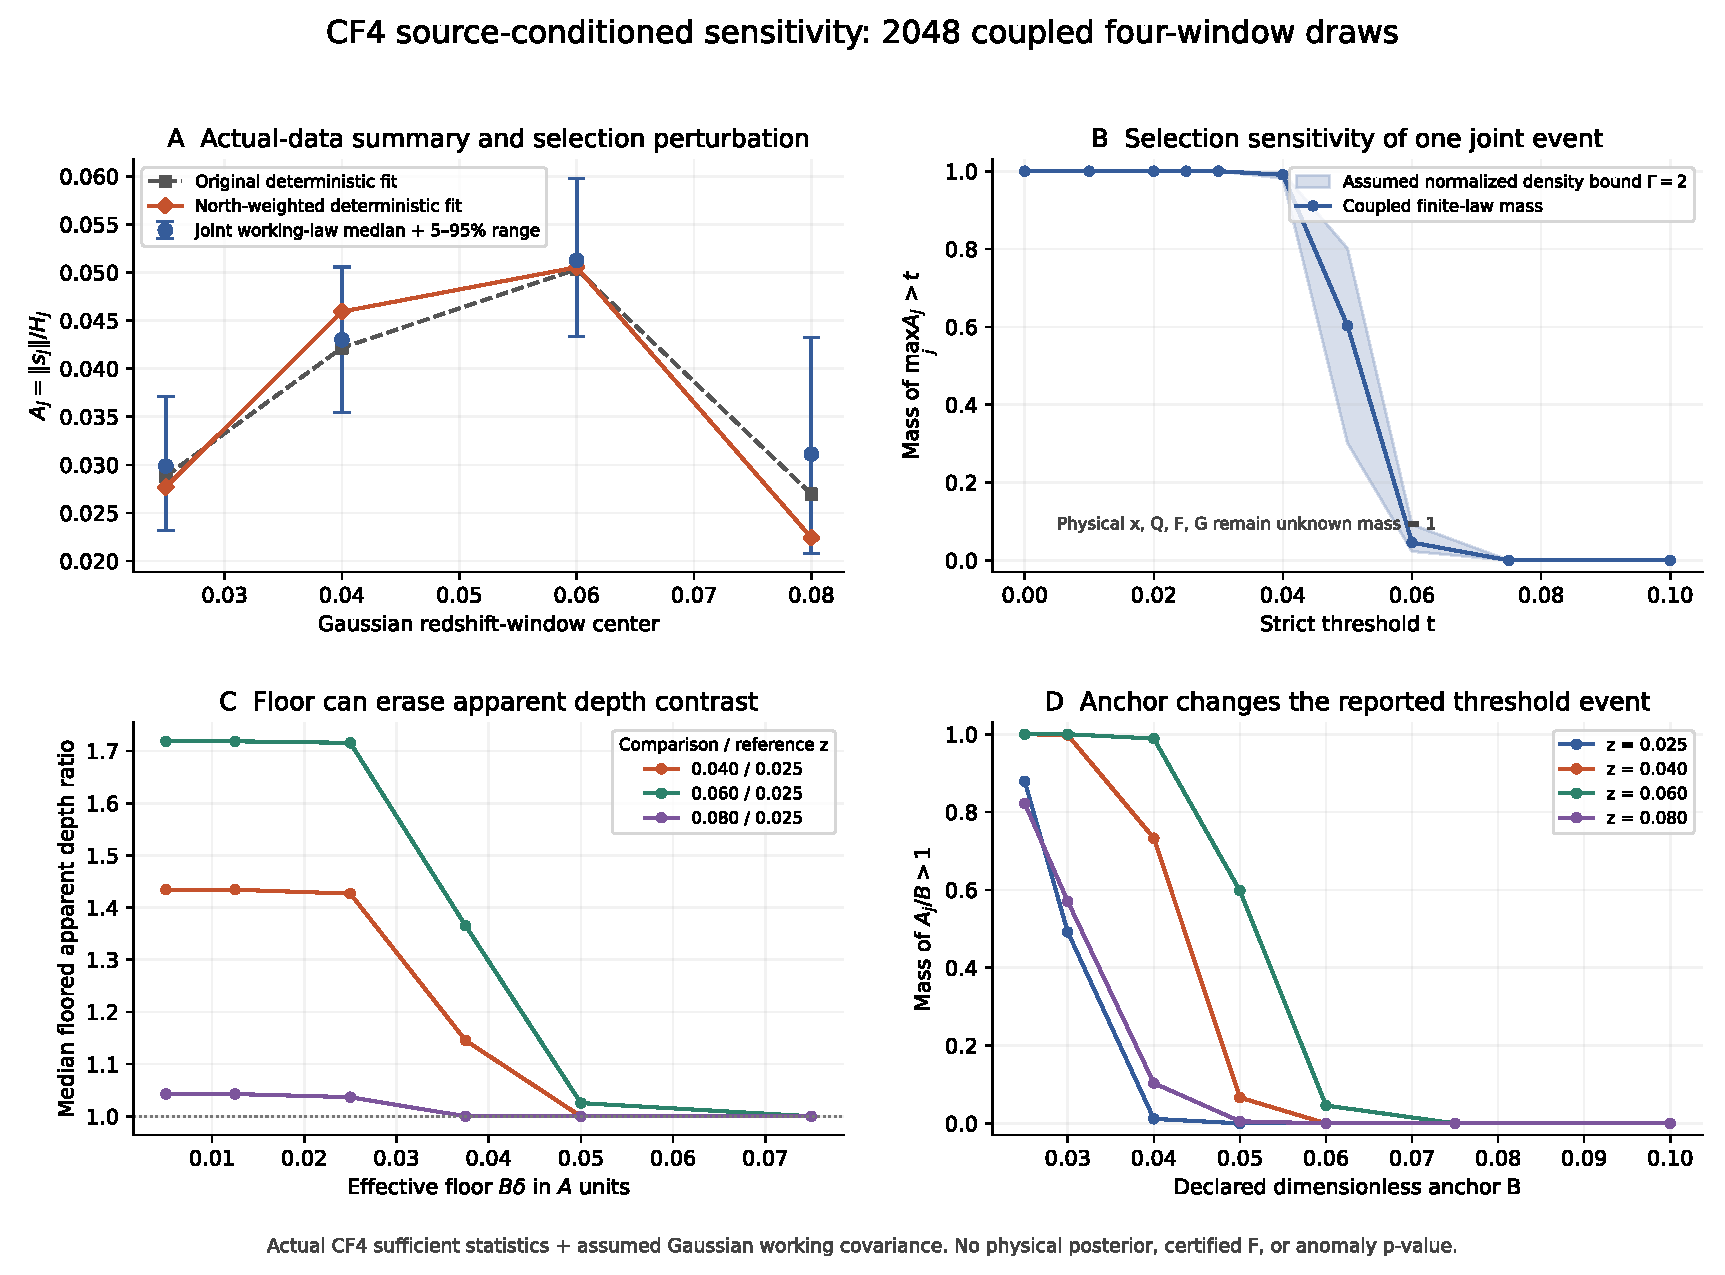
\includegraphics[width=.95\textwidth,height=.75\textheight,keepaspectratio]{figures/coupled_functionals.pdf}
\caption{Functional sensitivity of the separate four-window apparent Hubble-rate carrier. The blue quadrature summary in panel A and the summaries in panels B--D use the same retained 2048 coupled quadrature atoms and full cross-window covariance. Panel A also shows the deterministic baseline and north-weighted fits as estimator comparisons. The north-weighted covariance is unavailable, so these fits do not supply an alternative 2048-atom law or an uncertainty law for their difference. The apparent tensor norm, declared anchor, positive floor, and normalized density-ratio envelope have distinct roles. Finite-measure quantiles and masses are conditional on the stated reference construction; they do not constitute physical $Q_C$, $F$, $\Pi$, or $G_F$ measurements.}
\label{fig:functionals}
\end{figure}

Changing actual angular weights provides a different sensitivity check. The north-weighted apparent ratio differs from the baseline by approximately $-3.966\%$, $+8.918\%$, $+0.395\%$, and $-16.834\%$ across the four windows. Its covariance was not retained, so no new distribution is assigned to these shifts. Likewise, a stored method-deletion result supplies the norm of a tensor change rather than its direction. We use triangle-inequality outer intervals, not an invented deleted tensor. For deletion of the fundamental-plane family in the highest-redshift window, the retained interval for $A_j$ is $[0,0.06357699208]$. These calculations show source and estimator sensitivity on one catalogue.

\subsection{Unknown mass is not a zero-valued functional}

For a normalized finite measure with atom weights $p_i$, let $K$ be the indices where a functional is defined and known and let $U$ be the remaining indices. If $a_t=\sum_{i\in K}p_i\ind\{q_i>t\}$ and $u=\sum_{i\in U}p_i$, unrestricted completion of the unknown event indicators gives
\begin{equation}
 a_t\leq\Pi_{\mu,q}(t)\leq a_t+u.
 \label{eq:unknownmass}
\end{equation}
The two endpoints are attainable for unconstrained binary completions. Functional range restrictions can make them conservative rather than sharp; an eligible $F\leq1$, for example, cannot exceed one. A domain failure need not admit any physical completion at all. We therefore record domain failure separately from a defined but unmeasured value.

The present apparent carrier does not qualify physical $x_C$, $Q_C$, $F$, or $G_F$ on any atom. Its physical unknown mass is one. The generic interval $[0,1]$ records absence of a qualified physical event law, not a measured broad posterior and not a claim of physically sharp attainability at every threshold. Renormalizing only known values would instead condition on being known, changing the question. Ordered exceedance thresholds must also share one completed value per atom, so arbitrary independent choices from their marginal intervals need not define a possible exceedance curve.
